
% JuliaCon proceedings template
\documentclass{juliacon}
\setcounter{page}{1}

\begin{document}

% **************GENERATED FILE, DO NOT EDIT**************

\title{BlankLocalizationCore.jl: implementing blank localization in Julia}

\author[1, 2]{Tamás Cserteg}
\author[1]{András Kovács}
\author[1, 3]{József Váncza}
\affil[1]{EPIC Centre of Excellence, HUN-REN Institute for Computer Science and Control (SZTAKI), Budapest H-1111, Hungary}
\affil[2]{Doctoral School of Informatics, ELTE Eötvös Loránd University, Budapest H-1117, Hungary}
\affil[3]{Department of Manufacturing Science and Technology, Budapest University of Technology and Economics, Budapest H-1111, Hungary}

\keywords{Julia, Optimization, Machining, Blank localization}

\hypersetup{
pdftitle = {BlankLocalizationCore.jl: implementing blank localization in Julia},
pdfsubject = {JuliaCon 2022 Proceedings},
pdfauthor = {Tamás Cserteg, András Kovács, József Váncza},
pdfkeywords = {Julia, Optimization, Machining, Blank localization},
}



\maketitle

\begin{abstract}

Blank localization (also known as workpiece referencing) is an essential task in machining.
In this step the geometric relation of the tool of a machine (mill, lathe etc.) and the workpiece(s) needs to be precisely established.
We introduced the concept of multi operation blank localization to address this task for drilling and milling scenarios in a semi-automated way.
The method processes measurement of the rough geometry and the machining CNC code to solve a convex quadratically constrained quadratic program (QCQP).
It gives an optimal solution for given machining allowance--tolerance error, providing a tool for the machinist to find the appropriate balance between the two.
The versatility and extensibility of the Julia language helped the development of this algorithm, materializing in the \texttt{BlankLocalizationCore.jl} package.
Its flexibility and ease of use make it an excellent research tool, that can be deployed in production as well.
\end{abstract}

\section{Introduction}
\label{sec:intro}
Cast parts may have small geometric variations from lot-to-lot, that need to be addressed before machining by altering the CNC code.
Current practices include human effort, which takes long time, possibly produces scrap and requires highly trained workers.
Automated methods exist for complex free-form parts like wind turbines, that are based on the measurement of the rough part and generate the machining code by mini-max/maxi-min optimization (\cite{tan:2014_UnconstrainedApproachBlank}, \cite{ding:2021_CoarsefineOptimizationMethod}).
Multi operation blank localization was introduced in~\cite{cserteg:2023_Annals} focusing on drilling and milling.
These machining operations are among the most used ones, therefore the method is applicable for a wide range of products.
The method and its implementation was developed together, which required a language with support of easy prototyping and wide variety of tools.
For exactly these reasons chose we the Julia language~\cite{bezanson2017julia}.

%TODO: ez túl sok helyet foglal
\iffalse
The paper is structured as follows: the multi operation blank localization algorithm is introduced briefly in Sec.~\ref{sec:algo}, followed by the requirements and needs showed up during development in Sec.~\ref{sec:req} and the solutions of those problems in Sec.~\ref{sec:approach}.
Finally a short example is given in Sec.~\ref{sec:results} and the paper is concluded in Sec.~\ref{sec:conclusion}.
\fi

\section{Multi operation blank localization}
\label{sec:algo}

The goal of the algorithm is to find the optimal part zero for each feature group of a workpiece.
These feature groups could be for example drilled holes on the same side of the part, whose drilling positions are defined relative to a common reference (the part zero).
Features in a feature group can moved only together as a group, but feature groups can be moved separately.
The to-be-machined features (short: machined features) need to be aligned with the előgyártmány feauterök (called rough features) in a way, that a minimum machining allowance is ensured and the distance tolerance between features is respected.
Former encodes the requirement, that material needs to be removed to ensure proper surface finish and is described for a feature as the smallest thickness of material to be removed.
The distance tolerance between features is modeled as a lower-upper bound for the distance of two features.
As feature groups move together, only inter-group tolerances need to be considered.
Fig.~\ref{fig:hatfig} shows two feature groups with their part zeros as well as the tolerances between features.

\begin{figure}[b]
	\centerline{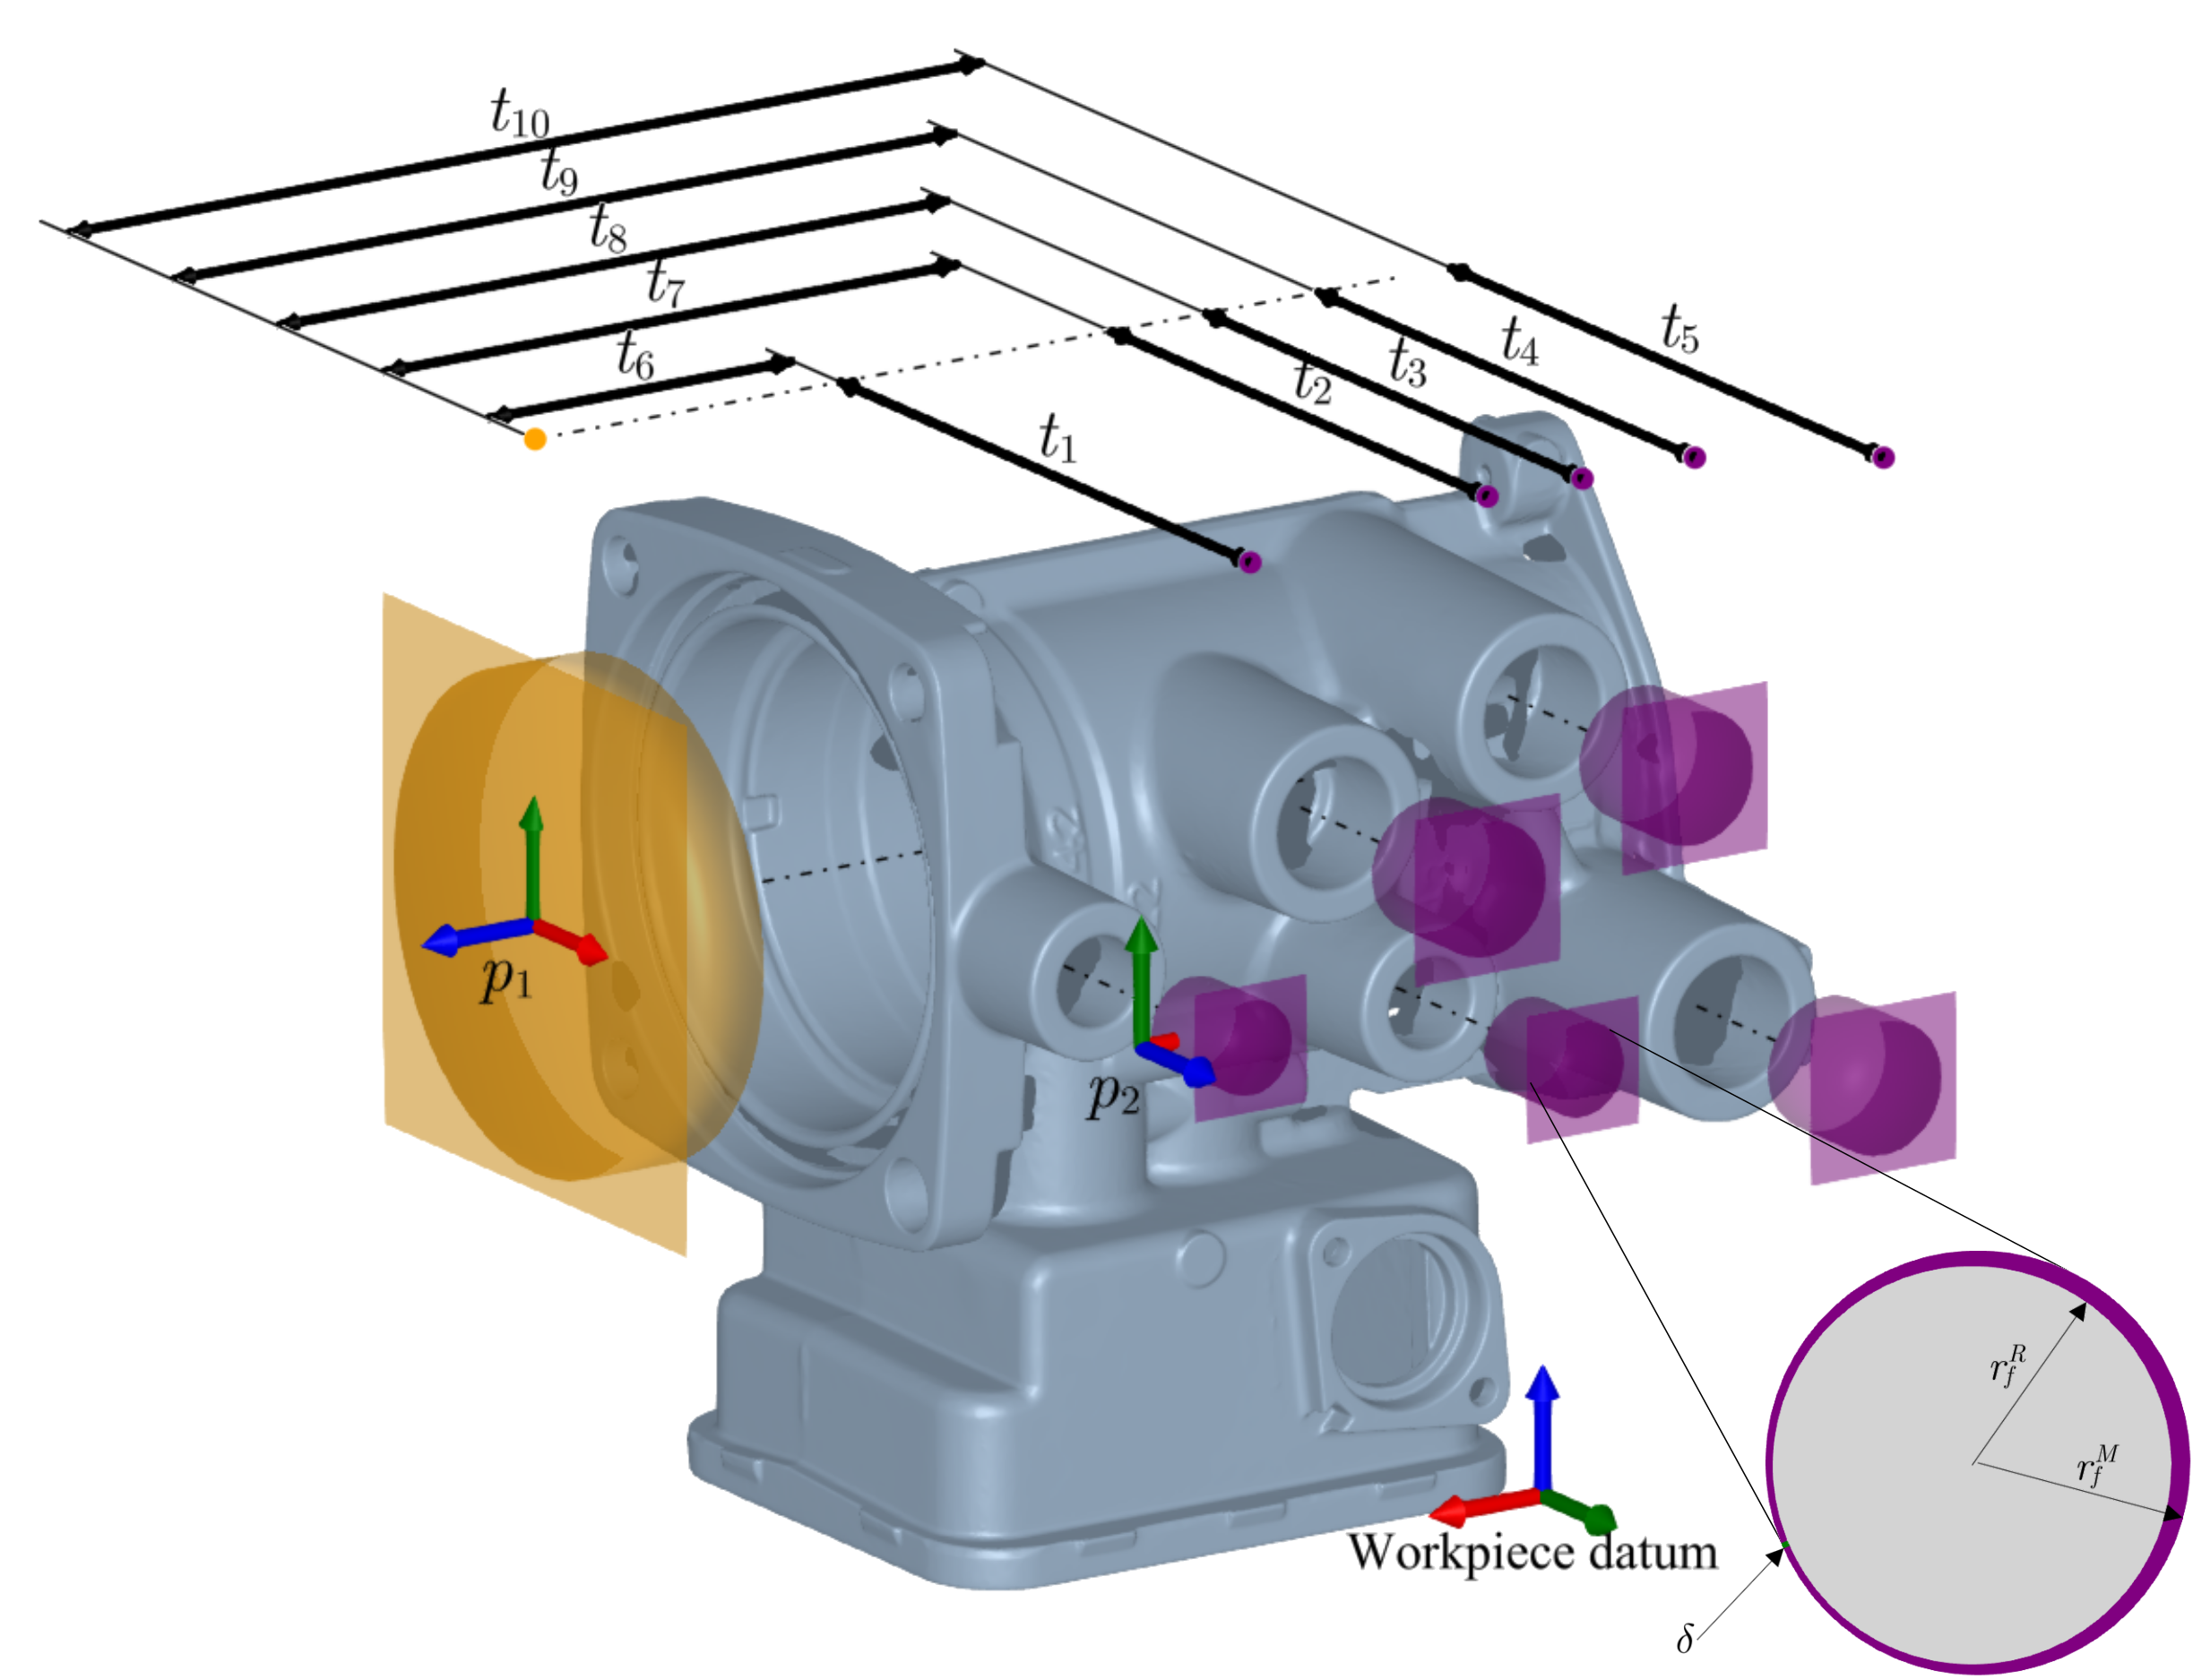
\includegraphics[width=0.9\columnwidth]{cirp-annals-2023-figure-2.png}}
	\caption{Measured part with two machined feature groups and tolerances between them. $r^M$ and $r^R$ denote the machined and rough radii of a feature, while $\delta$ the machining allowance \cite{cserteg:2023_Annals}.}
	\label{fig:hatfig}
\end{figure}

Inputs of the algorithm are the measurements of the rough part, the machining CNC code for each feature (relative to the corresponding part zero), the tolerance ranges for the features and the minimum machining allowance parameter.
The output will be the position of the optimal part zeros, where optimal means the lowest average tolerance error at the given allowance value.

Measurements of the rough parts can be obtained with a variety of instruments, including coordinate measurement machines (CMM), laser scanners, measurement arms, etc.
The two main representations that these devices create are primitive geometries (cylinders, planes, etc.) and free-form geometries in the form of point cloud or triangulated mesh.
These measurements are fed into the optimization model, which is a convex quadratically constrained quadratic program (QCQP).
Details of the optimization model can be found in the papers \cite{cserteg:2023_Annals} and \cite{cserteg:2023_CMS}.
%TODO: ide kéne még egy bekezdés arról, hogy mi is a modell?
% a mérések alapján -> QCQP ????
% a free-form / primitive-ről sem írtam még

\iffalse
The method gives engineers a tool to balance between machining allowance and tolerance error.
Former is 
Machining allowance is calculated for each feature as the smallest thickness of the material to be removed.
Tolerance error is defined for each dimensional tolerance record, that is defined between to features.
Their distance has a nominal value and upper-lower bounds.
The goal of the algorithm is to keep the tolerance distances close to the nominal value, while keeping a minimum machining allowance value.
\fi

\section{Approach}
\label{sec:approach}

During the development of the algorithm, we needed an environment (package) that supports the quick prototyping needs of research, while giving a stable background to validate the concept with our industry partner as well.
These needs include:
% (high-level, programozói igények nélkül, amit egy menedzser felsorolna):

\begin{itemize}
	\item A versatile type system for geometry representation. Especially regarding the differences of drilling/milling operations and free-form/primitive geometry representation.
	\item Easy-to-use interface for the optimization model.
	\item Support for importing geometries from a variety of measurement tools (CMM, laser scanner, measurement arm).
	\item Support for debugging, analyzing and visualizing the results.
%	\item Handling the differences of drilling and milling (hole and plane geometries).	
%	\item Model the problem, including geometry representaton, qcqp model building and solving, evaluation, visualization.
%	\item Modeling the different behavious of the geometries (holes, planes)
%	\item Handle two basic types of measurements: primitive or free-form.
%	\item Support for importing geometries: all kinds of measurement (expandable/extendable? type system for introducing new measurement types)
\end{itemize}

A flexible type system is designed to handle the different representations of geometries and features.
Abstract hole and plane geometries model the drilling and milling operations, while traits describe if a feature is using a free-form or a primitive representation.
An internal API (set of functions) is designed to access the relevant properties of the geometries (center point, radius, surface points, etc.).

This internal API is used when constructing the optimization model, utilizing the JuMP ecosystem~\cite{Lubin2023}.
With JuMP's excellent design, coding the optimization model was as easy as repeating the mathematical model in Julia.
Other advantage of the JuMP ecosystem is, that solvers can be easily swapped out if needed.
For development, the FICO Xpress solver was used (with academic license), but our industry partner could use the Ipopt or SCIP solvers without issue.
Using the internal API gives the advantage, that new geometry representations can be quickly used with the optimization model by just implementing a new type and a set of functions.

As mentioned earlier, important requirement was to handle the output formats of many different devices.
Every measurement instrument comes with its own processing software and export formats, not necessarily designed for interoperability.
As a result, we needed to write (or use) parsers for different text and tabular formats.
%The measurement results are read into their own respective type that implements the internal API, which means that 

The geometric computations are implemented with the help of the \texttt{Meshes.jl} package, which enabled us to easily visualize the geometries and results from the beginnings.
See Fig.~\ref{fig:hatfig} for an example.


\iffalse
Tasks are defined in the workpiece coordinate frame (called workpiece datum).
Two types of geometries need to be aligned: rough and machined. Currently the algorithm, thus the implementation supports two types of features: holes and planes. 
A flexible type system is implemented: abstract types are defined and all methods act on them, so implementing a new geometry type (for example to handle point cloud measurement of a rough hole) means defining the type and those methods.
All other functionality of the package are working automatically: setting up the optimization model, solving it, evaluating the results in details and visualizing the geometries.
\fi


\section{Results and future work} %TODO: or Example
\label{sec:results}

Fig.~\ref{fig:pareto} shows the allowance-tolerance pairs for an experiment from our paper.

\begin{figure}[b]
	\centerline{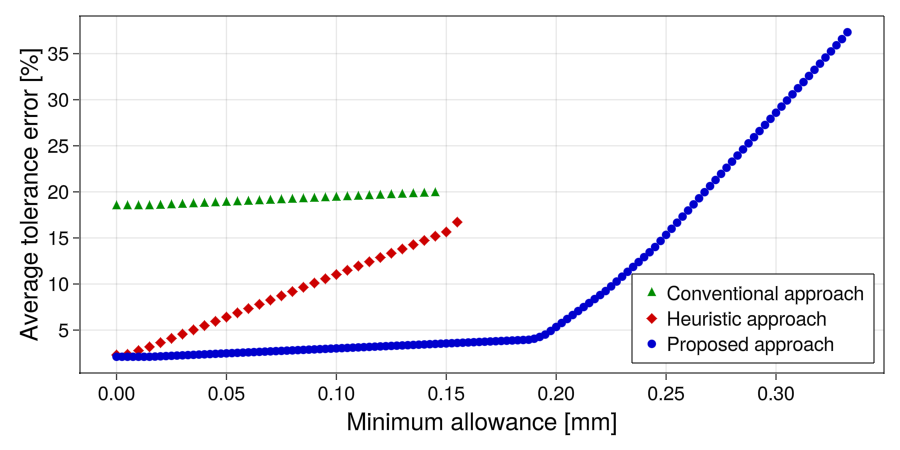
\includegraphics[width=0.9\columnwidth]{pareto-new-label.png}}
	\caption{Balancing the machining allowance and the tolerance error \cite{cserteg:2023_Annals}.}
	\label{fig:pareto}
\end{figure}


Preliminary results were first published in \cite{cserteg:2023_DigitalTwinAssisted}.
A journal paper describes the original algorithm \cite{cserteg:2023_Annals}, and a conference paper details the modifications for free-form surfaces \cite{cserteg:2023_CMS}.

Future plans for the package and the method itself include an overhaul of the tolerance modeling scheme.
Currently only dimensional tolerances are handled, but it should be discovered if more GD\&T tolerances can be incorporated into the model.
The methodology currently only supports cylinders and planes, thus drilling and milling.
It is a future research direction to extend the handled machining operations for example to turning.

%TODO: future works
% - tolerance modeling
% - discover other machining operations (turning)
% - add more examples to docs


\section{Acknowledgments}
%TODO: CMS másolása
This research has been supported by the National Laboratory for Autonomous Systems RRF-2.3.1-21-2022-00002 and the ED\_18-2-2018-0006 grants of the NRDIO.

% **************GENERATED FILE, DO NOT EDIT**************

\bibliographystyle{juliacon}
\bibliography{ref.bib}


\end{document}

% Inspired by the International Journal of Computer Applications template
